\documentclass{article}

\usepackage{graphicx}
\usepackage{tikz}
\usepackage{tikzsymbols}
\usetikzlibrary{calc,patterns,shapes.geometric}
\pagestyle{empty}
\usepackage[margin=0pt]{geometry}
\geometry{papersize={14in,12in}}

\def\centerarc[#1](#2)(#3:#4:#5){\draw[#1] ($(#2)+({#5*cos(#3)},{#5*sin(#3)})$) arc (#3:#4:#5);}

\begin{document}
	\begin{figure}
		\centering
		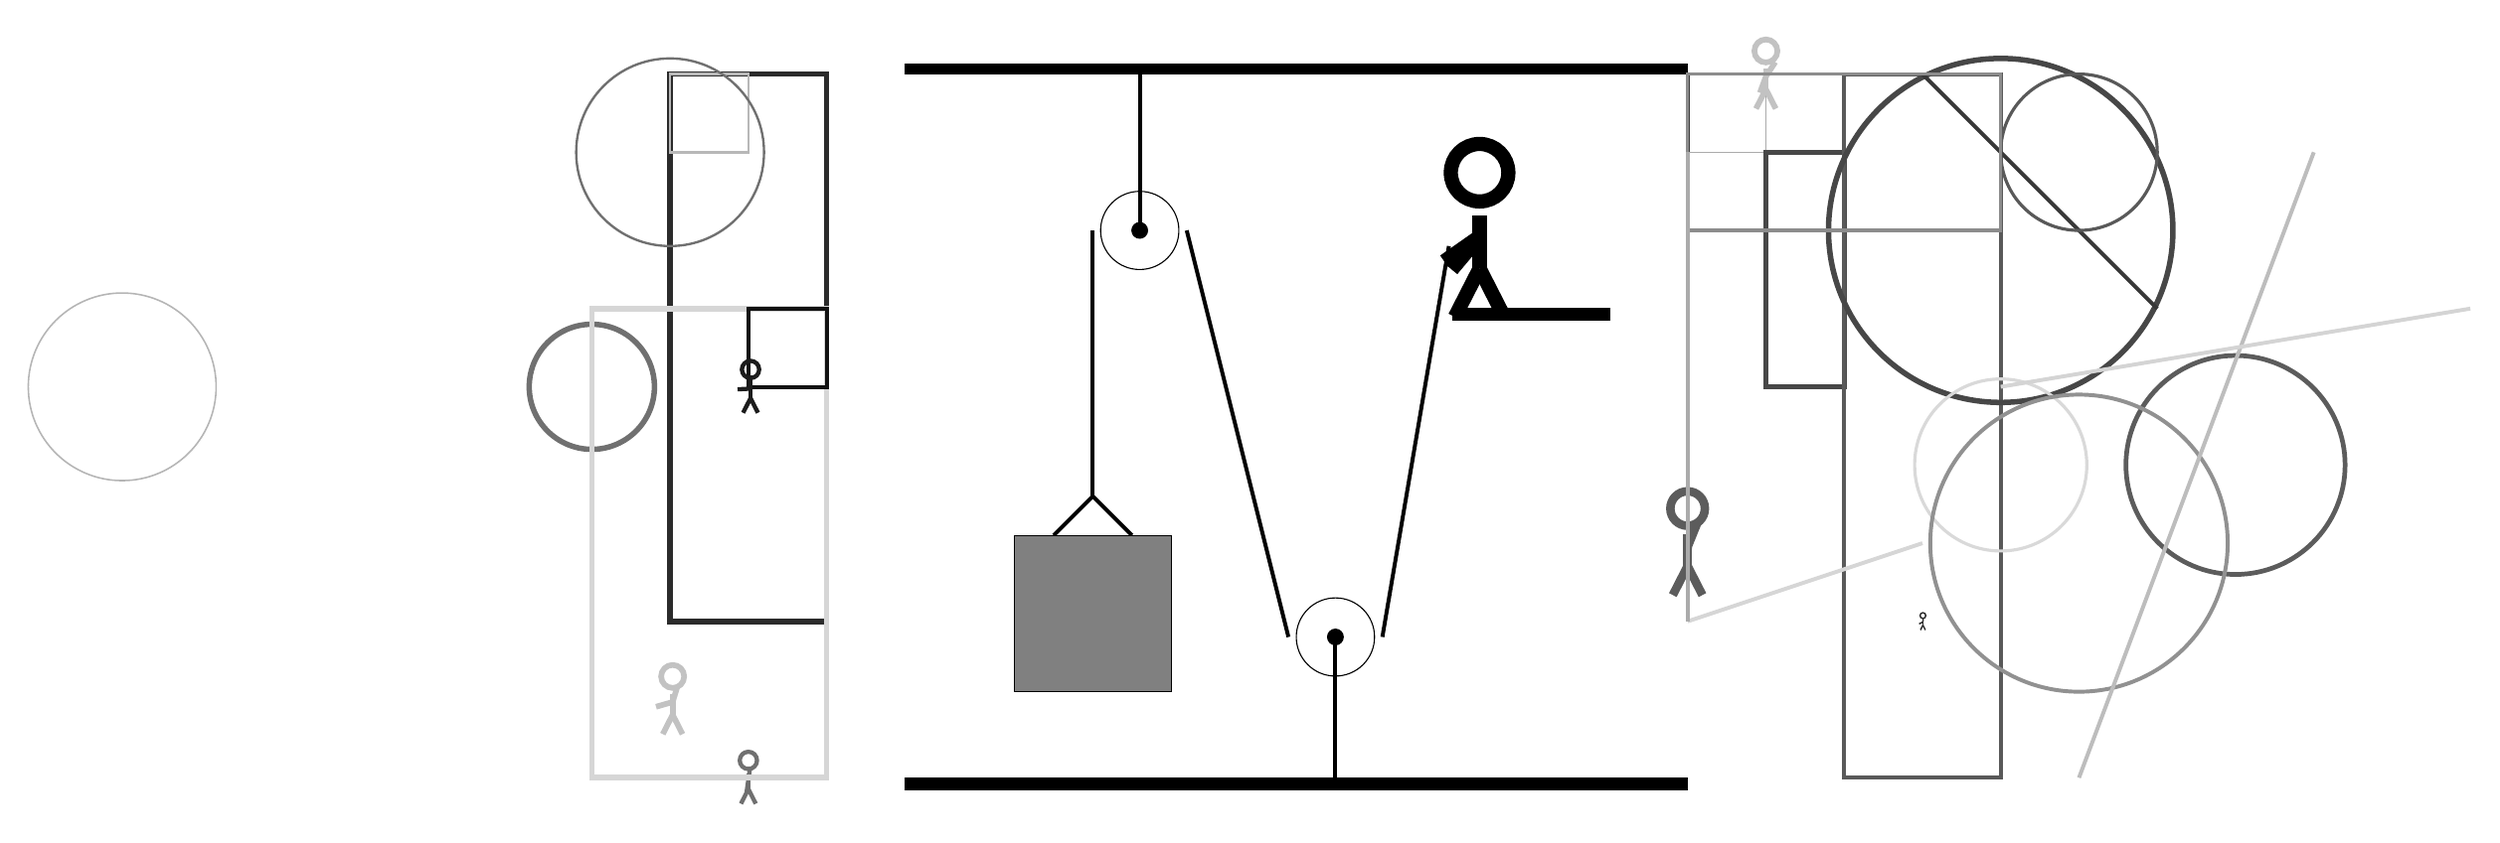
\begin{tikzpicture}
			%%%%% START %%%%%
			
			\draw[fill=black] (-2, 9) rectangle (8, 9.125);
			
			\draw (3.5, 1.8) circle (0.5);
			\draw[fill=black] (3.5, 1.8) circle (0.1);
			\draw[line width=0.5mm] (3.5, 1.8) -- (3.5, 0);
			
			\draw (1, 7) circle (0.5);
			\draw[fill=black] (1, 7) circle (0.1);
			\draw[line width=0.5mm] (1, 9) -- (1, 7);
			
			\node[line width=0.4mm, color=black!56] at (-4, 0) {\Strichmaxerl[3][82][82]};
			
			\draw[line width=0.2mm, color=black!33] (9, 9) rectangle (8, 8);
			\draw[line width=0.6mm, color=black!72] (10, 8) rectangle (9, 5);
			\draw[line width=0.3mm, color=black!93] (10, 3) rectangle (10, 5);
			
			\draw [line width=0.6mm, color=black!64](15, 4) circle (1.4);
			\draw[line width=0.5mm, color=black!65] (10, 0) rectangle (12, 9);
			
			\draw [line width=0.7mm, color=black!72](12, 7) circle (2.2);
			
			\node[line width=0.2mm, color=black!83] at (11, 2) {\Strichmaxerl[1][27][86]};
			\draw[line width=0.5mm, color=black!78](11, 9) -- (14, 6);
			
			\draw [line width=0.4mm, color=black!65](13, 8) circle (1.0);
			
			\draw[line width=0.7mm, color=black!83] (-3, 9) rectangle (-5, 2);
			
			\node[line width=0.6mm, color=black!64] at (8, 3) {\Strichmaxerl[6][89][68]};
			\node[line width=0.6mm, color=black!24] at (9, 9) {\Strichmaxerl[4][70][57]};
			
			\draw [line width=0.7mm, color=black!56](-6, 5) circle (0.8);
			\draw[line width=0.5mm, color=black!76](8, 8) -- (8, 9);
			\draw[line width=0.7mm, color=black!16] (-3, 0) rectangle (-6, 6);
			
			\draw [line width=0.4mm, color=black!15](12, 4) circle (1.1);
			\draw[line width=0.3mm, color=black!28] (-4, 8) rectangle (-5, 9);
			\draw [line width=0.5mm, color=black!43](13, 3) circle (1.9);
			\draw[line width=0.5mm, color=black!16](11, 3) -- (8, 2);
			\draw[line width=0.5mm, color=black!26](13, 0) -- (16, 8);
			
			\draw[line width=0.5mm, color=black!93] (-4, 5) rectangle (-3, 6);
			\draw[line width=0.4mm, color=black!45] (8, 9) rectangle (12, 7);
			\draw[line width=0.5mm, color=black!17](12, 5) -- (18, 6);
			\draw[line width=0.5mm, color=black!33](8, 8) -- (8, 2);
			
			\draw [line width=0.3mm, color=black!56](-5, 8) circle (1.2);
			
			\node[line width=0.2mm, color=black!24] at (-5, 1) {\Strichmaxerl[4][16][73]};
			\node[line width=0.6mm, color=black!89] at (-4, 5) {\Strichmaxerl[3][3][90]};
			\draw [line width=0.2mm, color=black!29](-12, 5) circle (1.2);
			
			\draw[line width=0.5mm](-0.1, 3.1) --  (0.4, 3.6) -- (0.9, 3.1);
			\draw[fill=black!50] (-0.6, 3.1) rectangle (1.4, 1.1);
			
			\draw[line width=0.5mm](0.4, 7) -- (0.4, 3.6);
			\centerarc[line width=0.5mm](1, 7)(180:0:0.6)
			\draw[line width=0.5mm](1.6, 7) -- (2.9, 1.8);
			\centerarc[line width=0.5mm](3.5, 1.8)(180:360:0.6)
			\draw[line width=0.5mm](4.1, 1.8) -- (4.95, 6.8);
			
			\node at (5.3, 7) {\Strichmaxerl[10][35][-130]};
			\draw[fill=black] (5, 6) rectangle (7, 5.85);
			
			\draw[fill=black] (-2, 0) rectangle (8, -0.15);
			
			%%%%% END %%%%%
		\end{tikzpicture}
	\end{figure}	
\end{document}